\subsection{
  Replies to comments received from Neil McCauley - Jan. 06, 2013 }

\begin{enumerate}

%........................................................................................................
\vspace{5 mm}
\item
{\em
  ``The non 2-3 oscillation parameters are fixed to 2012 PDG values. 
  It would be a good idea to put a table with these values and their uncertainties into the document.''
}\\
\\
The values are shown in Sec.\ 4.1.2 but it is not made clear, in that context, that they are 
the 2012 PDG values. Uncertainties in these parameters are not quoted.
A table will be added in version 2 of T2K-TN-141 as suggested.

%........................................................................................................
\vspace{5 mm}
\item
{\em
  ``What is the impact of removing the upper limit of $sin^2(2\theta_{23})<1$ on the fit? Can we see the results?''
}\\
\\
Please see the reply to a similar question asked by Boris P.

%........................................................................................................
\vspace{5 mm}
\item
{\em
  ``Does the fit have any sensitivity to the choice of upper and lower limits on ${\Delta}m^2$?''
}\\
\\
The lower limit on $|{\Delta}m^2_{32}|$ was changed from 
$1 \times 10^{-3} eV^2/c^4$ to $1 \times 10^{-4} eV^2/c^4$
and the upper limit was changed from 
$6 \times 10^{-3} eV^2/c^4$ to $6 \times 10^{-2} eV^2/c^4$.
The best-fit values were unchanged.

%........................................................................................................
\vspace{5 mm}
\item
{\em
  ``Why do you limit systematics to +- 1 sigma? 
  We have enough systematics that we should expect to see systematics outside the 
  1 sigma range by random chance, this is true even in the reduced systematics fit. 
  What it the impact of removing this limit?''
}\\
\\
There was a typing mistake in T2K-TN-141v1.
Systematic parameters included in the oscillation fit are in fact constrained to be in the range
[-5$\sigma$, +5$\sigma$].  The only exception, as mentioned in the text (footnote 5), 
is the systematic parameter $f_{SF}$ which parameterizes the uncertainty on nuclear modelling. 
This is constrained to be in the 
range [0,1] which is the entire allowed range for it.

%........................................................................................................
\vspace{5 mm}
\item
{\em
  ``Figs 24,26,26 Figure referenced in the table is figure 259, but looks like it should be figure 23.''
}\\
\\
In version 2 of T2K-TN-141, the latex referencing will be fixed.

%........................................................................................................
\vspace{5 mm}
\item
{\em
  ``2 systematics from the banff are in the 8 important ones, parameters 16 and 18. 
  I suggest a reminder in the text at this point about what these parameters are. 
  I think ma and cc normalisation, but I'm not sure. Please clarify.''
}\\
\\
The BANFF parameter numbering scheme used is shown in Table 6.
Parameter 16 is the CCQE axial mass parameter, $M_{A}^{QE}$ and 
parameter 18 is the CCQE normalization in the true energy range 0 - 1.5 GeV.
As suggested, 
a reminder will be added in the text of version 2 of T2K-TN-141 when the 8 most important systematic
parameters are listed.

%........................................................................................................
\vspace{5 mm}
\item
{\em
  ``The banff parameters are strongly correlated with each other is it safe to separate 
  them out to be treated as individuals.
  For example the cross section parameters play off against the flux parameters, 
  so I'm not sure you can safely just vary one or the other independently post banff. 
  Please comment.''
}\\
\\
In the `2+8' fit, only 2 of the 23 BANFF parameters are included in the 8 systematic
parameters we fit. However, the correlations between the BANFF parameters are respected.
Although 21 of the BANFF parameters are not allowed to float {\em independently},
their values do change as a result of changing the values of the 2 BANFF parameters we fit.
Let j be a index which runs over the set of BANFF parameters we fit (the ones we allow to 
float independently), and i be an index which runs over the set of BANFF parameters we do not fit.
When parameters $f^{banff}_j$ float, then parameters $f^{banff}_i$ are automatically adjusted,
due to their correlations, by
\begin{equation} \nonumber
\Delta f^{banff}_i = \sum_j f^{banff}_j C_{ij}
\end{equation}
where $C_{ij}$ is the BANFF covariance matrix.
In addition, when calculating the BANFF penalty term, the full BANFF matrix is used.
A clarification of this will be added in version 2 of T2K-TN-141.
The validitity of the approach can be judged from the fact that the `2+8' and `2+N'
results are very similar.

Also it should be noted that all parameter correlations are fully taken into account 
when the toy MC experiments are generated, and this is true for all fit methods.

%........................................................................................................
\vspace{5 mm}
\item
{\em
  ``Figure 45/46. Would I be correct in assuming the y axis on the lower plot is in units 
  of number of events? Please clarify. Could you also show the fractional differences.''
}\\
\\
The lower plot shows the absolute differences between the two best-fit predictions.
As you say, the y axis has units of number of events.
A clarification will be added in the caption.
Also, plots showing the fractional differences will be added in version 2 of T2K-TN-141.

%........................................................................................................
\vspace{5 mm}
\item
{\em
  ``Figure 57/58 and similar plots. Could we use our own contour for reference not that of minos. 
  It's over the range of our own contour that any differences will matter.''
}\\
\\
Indeed. 
But when Figures 57/58 are discussed in the paper, no T2K contours have been shown yet.
Introducing the T2K contours at that point would disturb the flow of the paper.
The region shown in the plots includes a much larger parameter space than that included 
in the T2K contours which are shown later in the note.
The MINOS contours are shown in all similar comparisons,
especially since it is the MINOS results which were used to guide the selection 
of grid points for the sensitivity and systematic studies shown in the paper.
The plot which best illustrates the similarity of the $\Delta\chi^2$ surfaces within 
the T2K confidence region is Fig.\ 69, which shows that the two
confidence regions are nearly identical.

For your reference, the requested plot is shown below.

\begin{figure*}[htb]
\begin{minipage}[t]{0.48\linewidth}
\center
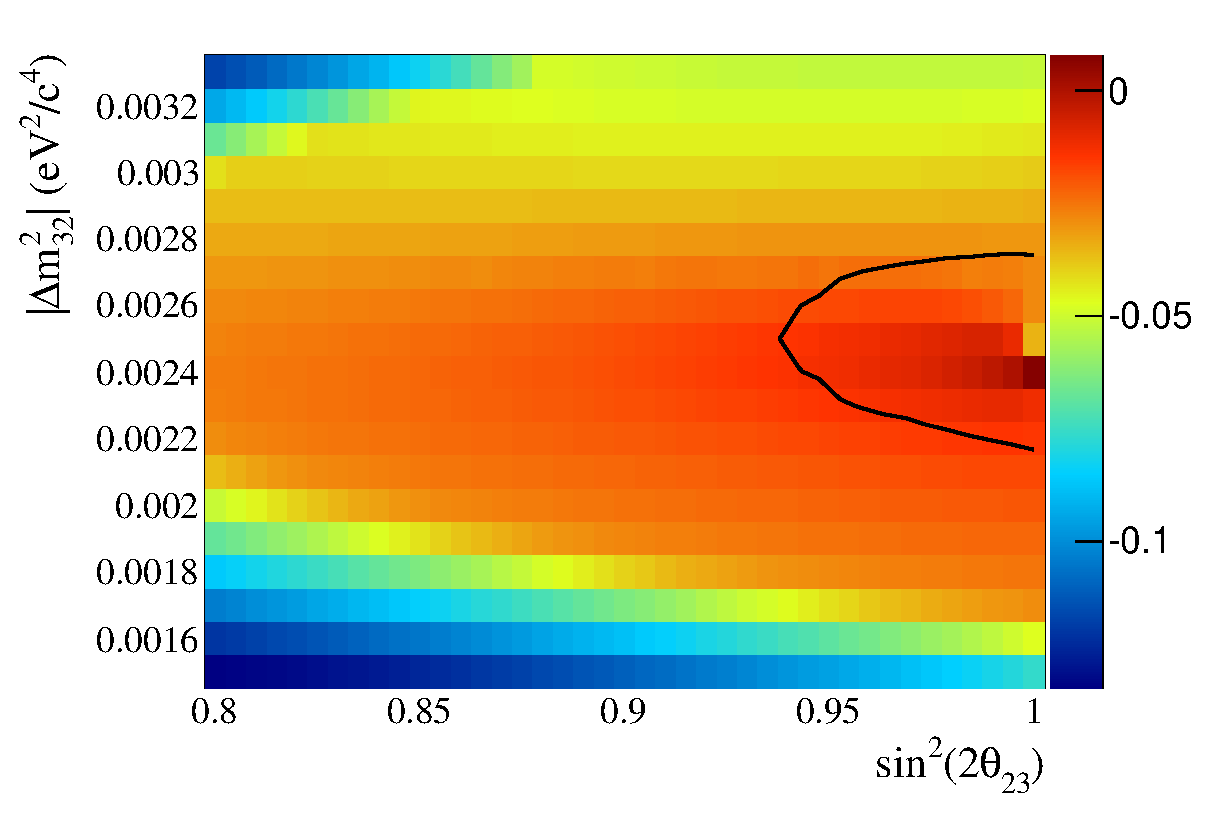
\includegraphics[width=20pc]{./images/compare_2all_28_dchisqdiff_nM8OnP8O2_t2kcont}
\caption {
  Fractional difference between the $\Delta\chi^2$ surfaces
  obtained from the `2+N' and `2+8' fits to the Run 1+2+3 dataset.
  The fractional difference is calculated as 
  2 $\times$ ($\Delta\chi^2$(`2+N')-$\Delta\chi^2$(`2+8')) / $\Delta\chi^2$(`2+N')+$\Delta\chi^2$(`2+8')).
  The T2K Run 1+2+3 `2+8' FC 90\% CL region is shown for reference.
}
\label{fig:results_dchisq_fracdiff_run123}
\end{minipage}
\hspace{0.06\linewidth}
\begin{minipage}[t]{0.48\linewidth}
\center
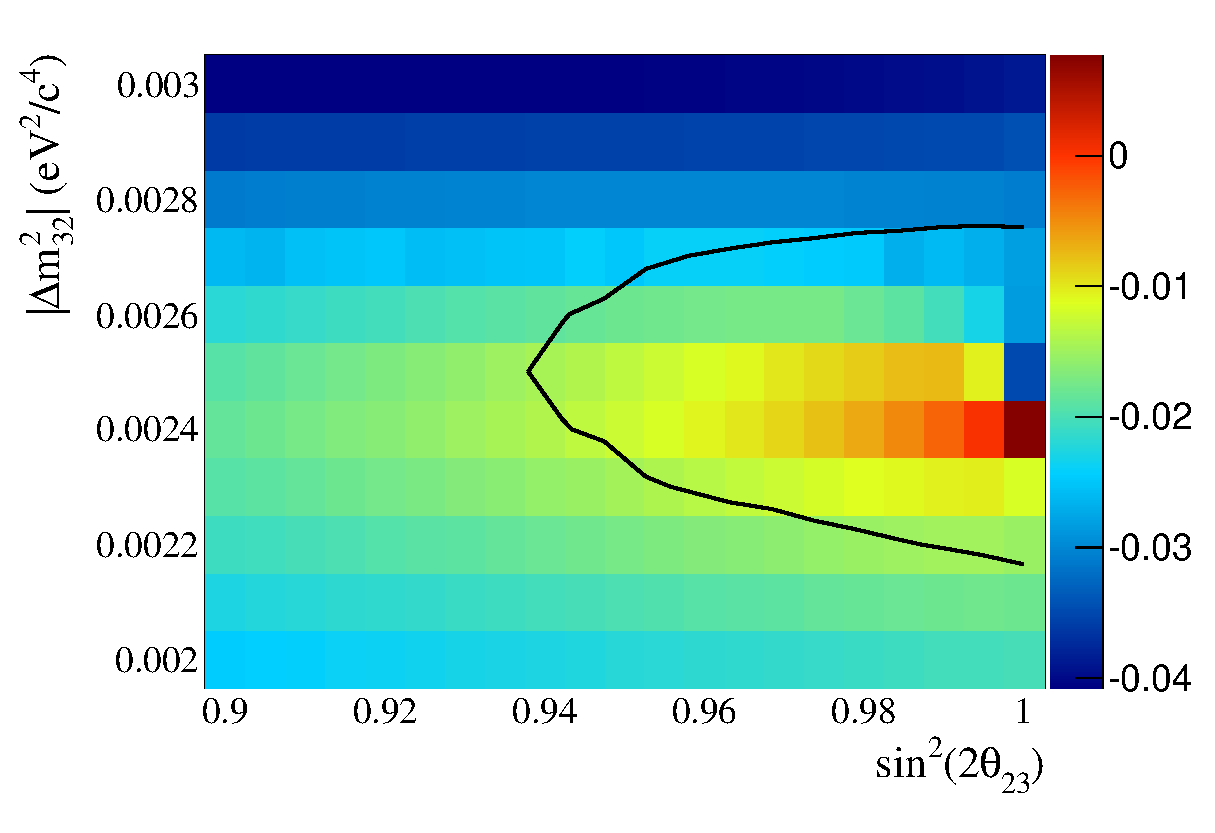
\includegraphics[width=20pc]{./images/compare_2all_28_dchisqdiff_nM8OnP8O2_zoom_t2kcont} 
\caption {
  As in Fig.\ \ref{fig:results_dchisq_fracdiff_run123} but zoomed into the area of the 90\% CL region.
}
\label{fig:results_dchisq_fracdiff_run123_zoom}
\end{minipage}
\end{figure*}


%........................................................................................................


\end{enumerate}
